\section{OPTIMISATION OF EVENT SELECTION}  

In the CMS experiment there are many proton-proton beams collisions which produce a lots of detected events data.
Since there is a huge rate (40MHz) of bunch crossing it is impossible to save and analize all of the data.
The event selection is an essential stage in the OMTF and it is being done by a trigger.
The reduction of rate is achieved by rejecting these events that are unattractive in experiment.
So the trigger has to recontruct muon tracks in each event to make a so-called cut.
The cut consists on rejecting muons with tranverse momentum lower than a specified threshold value and accept that events with a bigger one.

In the Fig. \ref{eff} there is a plot of efficiency of trigger for a momentum cut set on 16 GeV/c vs transverse momentum of muons.
The efficency is defined as a ratio of number of accepted muons to number of all muons.
The ideal efficiency curve should look like a step function changing the efficiency value from 0 to 1 in the threshold value point.

There were performed tests of optimisation of event selection.
In this study were used data samples with simulated single muon events
The current event selecion algorithm is based on quality and PDF value.
The improved one takes into consideration diversity of efficiency of each reference layer and adds different relevance to PDF subvalues that depends on detector type.
The RPC detectors was devalued because of their poor spatial resolution, the weight for DT detectors was increased due to their excellent spatial resolution.
For CSC detectors there were no changes.
In the Fig. \ref{eff} there is plot of these two options of muon selecion in OMTF - actual and improved.
They are compared with the best possible efficiency for that case, that is known because it is plotted on simulated Monte Carlo data.

\begin{figure}[ht]
\centering
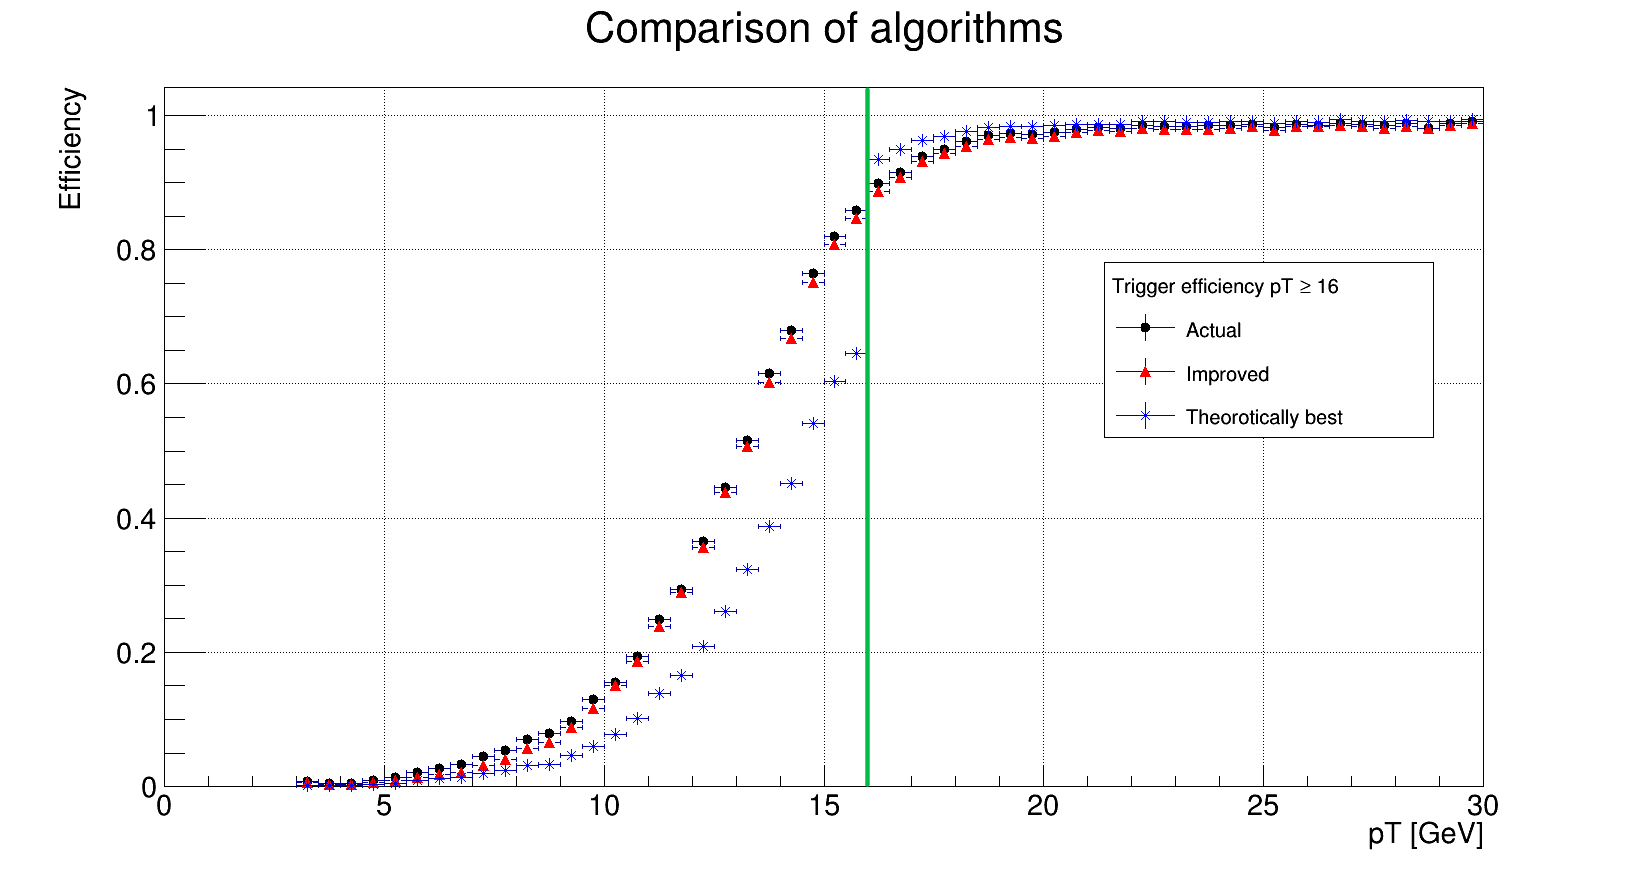
\includegraphics[width=0.7\textwidth]{Hist16.png}
\caption{Efficiency of different algorithms of events selection vs muon transverse momentum}
\label{eff}
\end{figure} 

The selection in the range below the momentum cut is very essential because it improves the purity of trigger.
It is important since low-energetic muons increase a difficulty of data analysis.
In the Fig. \ref{ratio} there is a plot of ratio of previous efficiencies that shows some improvement in range of low tranverse momentum.

\begin{figure}[ht]
\centering
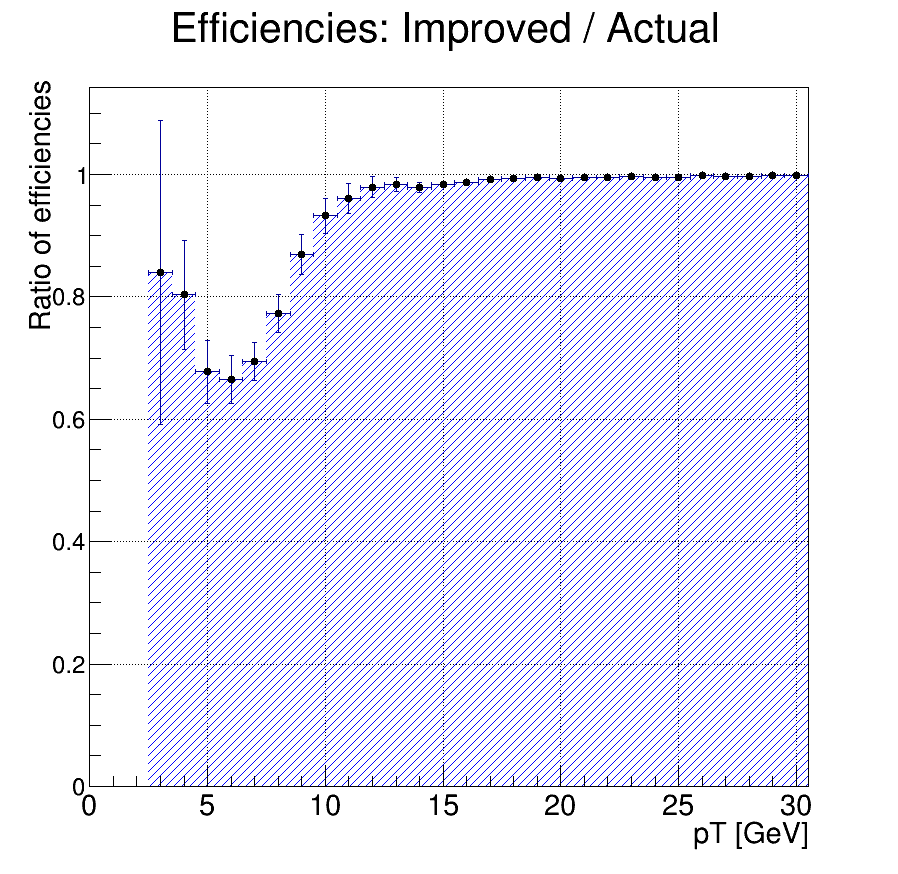
\includegraphics[width=0.4\textwidth]{Ratio16.png}
\caption{Ratio of improved efficiency and acutal efficiency. Muons with momentum in the range from 3 to 12 GeV are rejected in a better way.}
\label{ratio}
\end{figure} 

